% based on Model 2 of "Activity 10 - Class Design" by Helen Hu

\model{Class Design}

Classes are often used to represent abstract data types, such as \java{Color} or \java{Point}.
They are also used to represent objects in the real world, such as \java{CreditCard} (see next page) or \java{Person}.
%UML class diagrams summarize the attributes and methods of a class.

\begin{center}
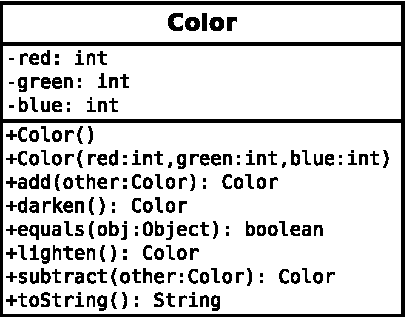
\includegraphics{Color.pdf}  % immutable
~~~~~
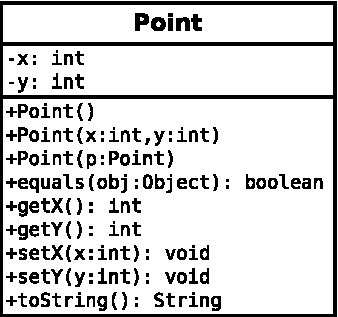
\includegraphics{Point.pdf}  % mutable
\end{center}

Classes generally include the following kinds of methods (in addition to others):
\begin{itemize}[itemsep=0pt]
\item \textbf{constructor} methods that initialize new objects
\item \textbf{accessor} methods (getters) that return attributes
\item \textbf{mutator} methods (setters) that modify attributes
\item \textbf{object} methods such as \java{equals} and \java{toString}
%\item \textbf{utility} methods which are generally static
\end{itemize}


\quest{20 min}


\Q Identify the constructors for the \java{Color} class. What is the difference between them? What arguments do they take?

\begin{answer}
There are two constructors: one that takes three integers for the RGB values, and other that takes a Color object. The latter is called a \emph{copy constructor}. Constructors do not return values.
\end{answer}


\Q Identify an accessor method in the \java{Point} class. 
\begin{enumerate}[itemsep=1pt]
\item Which instance variable does it get? \ans{{\tt this.x} or {\tt this.y}}
\item What arguments does the method take? \ans{none}
\item What does the method return? \ans{The value of \java{x} or \java{y}}
\end{enumerate}


\Q Identify a mutator method in the \java{Point} class.
\begin{enumerate}[itemsep=1pt]
\item Which instance variable does it set? \ans{{\tt this.x} or {\tt this.y}}
\item What arguments does the method take? \ans{The value of \java{x} or \java{y}}
\item What does the method return? \ans{nothing}
\end{enumerate}


\begin{center}
\textit{For the remaining questions, you will design a class that represents an individual's credit card.}
\bigskip\par
% https://www.bankofamerica.com/credit-cards/

\includegraphics{credit-card.png}
\end{center}


\Q List two or more attributes that would be necessary for this \java{CreditCard} class. For each attribute, indicate what data type would be most appropriate.

\begin{answer}[5em]
Answers may include \verb|number:long|, \verb|expire:Date|, \verb|name:String|, \verb|code:int|, etc.
\end{answer}


\Q When constructing (or updating) a \java{CreditCard} object, what values would you need to check? What are the valid ranges of values for each attribute?

\begin{answer}[5em]
The number should have 16 digits, dates need to have valid months and days, names should be at most 22 letters and not contain digits or other characters, code should be 3--4 digits.
\end{answer}


\Q List two accessor methods would be appropriate for the \java{CreditCard} class.
Include arguments and return values, using the same format as a UML diagram.

\begin{answer}[5em]
\begin{verbatim}
+getNumber(): long
+getExpire(): Date
+getName(): String
+getCode(): int
\end{verbatim}
\end{answer}


\Q List two mutator methods would be appropriate for the \java{CreditCard} class.
Include arguments and return values, using the same format as a UML diagram.

\begin{answer}[5em]
\begin{verbatim}
+setNumber(number:long): void
+setExpire(expire:Date): void
+setName(name:String): void
+setCode(code:int): void
\end{verbatim}
\end{answer}
